\documentclass[a4paper,10pt]{article}
%\documentclass[a4paper,10pt]{book}

\usepackage[dvipdfmx]{graphicx, color}
%\usepackage{folha}
\graphicspath{{image/}}

\usepackage{color}
\usepackage{array}
\usepackage{longtable}
\usepackage{alltt}
\usepackage{graphics}
\usepackage{vpp-nms}
%\usepackage{vpp}
\usepackage{makeidx}
\makeindex

\usepackage{colortbl}

\usepackage[dvipdfmx,bookmarks=true,bookmarksnumbered=true,colorlinks,plainpages=true]{hyperref}

%\AtBeginDvi{\special{pdf:tounicode 90ms-RKSJ-UCS2}}
\AtBeginDvi{\special{pdf:tounicode EUC-UCS2}}

\definecolor{covered}{rgb}{0,0,0}      %black
\definecolor{not-covered}{rgb}{1,0,0}  %red

\setcounter{secnumdepth}{6}
\makeatletter
\renewcommand{\paragraph}{\@startsection{paragraph}{4}{\z@}%
  {1.5\Cvs \@plus.5\Cdp \@minus.2\Cdp}%
  {.5\Cvs \@plus.3\Cdp}%
  {\reset@font\normalsize\bfseries}}
\makeatother

\renewcommand{\sf}{\sffamily \color{blue}}

\newcommand{\syou}{\texttt{<}}
\newcommand{\dai}{\texttt{>}}

%\include{Title}

%\pagestyle{empty}
\usepackage{fancyhdr}
\usepackage{lastpage} 
  \pagestyle{fancy} 
   \let\origtitle\title 
  \renewcommand{\title}[1]{\lfoot{#1}\origtitle{#1}}

  \rfoot{\today}
  \rhead{[\ \scshape\oldstylenums{\thepage}\ / %
      \scshape\oldstylenums{\pageref{LastPage}}\ ]}
  \cfoot{}


\begin{document}

% the title page
\title{VDM++ specification of calculating railway fare}
\author{Shin Sahara\\\\
Hosei University\\
}
%\institute{\pgldk \and \chessnl}
\date{\mbox{}}
\maketitle
\begin{abstract}
This is an example of industrial requirement specification.

This example calculates fare by distance using sequence of record.

\end{abstract}


%\setlength{\baselineskip}{12pt plus .1pt}
%\tolerance 10000
\tableofcontents
%\thispagestyle{empty} 

\section{Class Diagram}
\index{Class Diagram}

This is the class diagram of the VDM++ specification.
The layer of the class is on upper right of the class box.

\begin{figure}[h]
	\centering
	{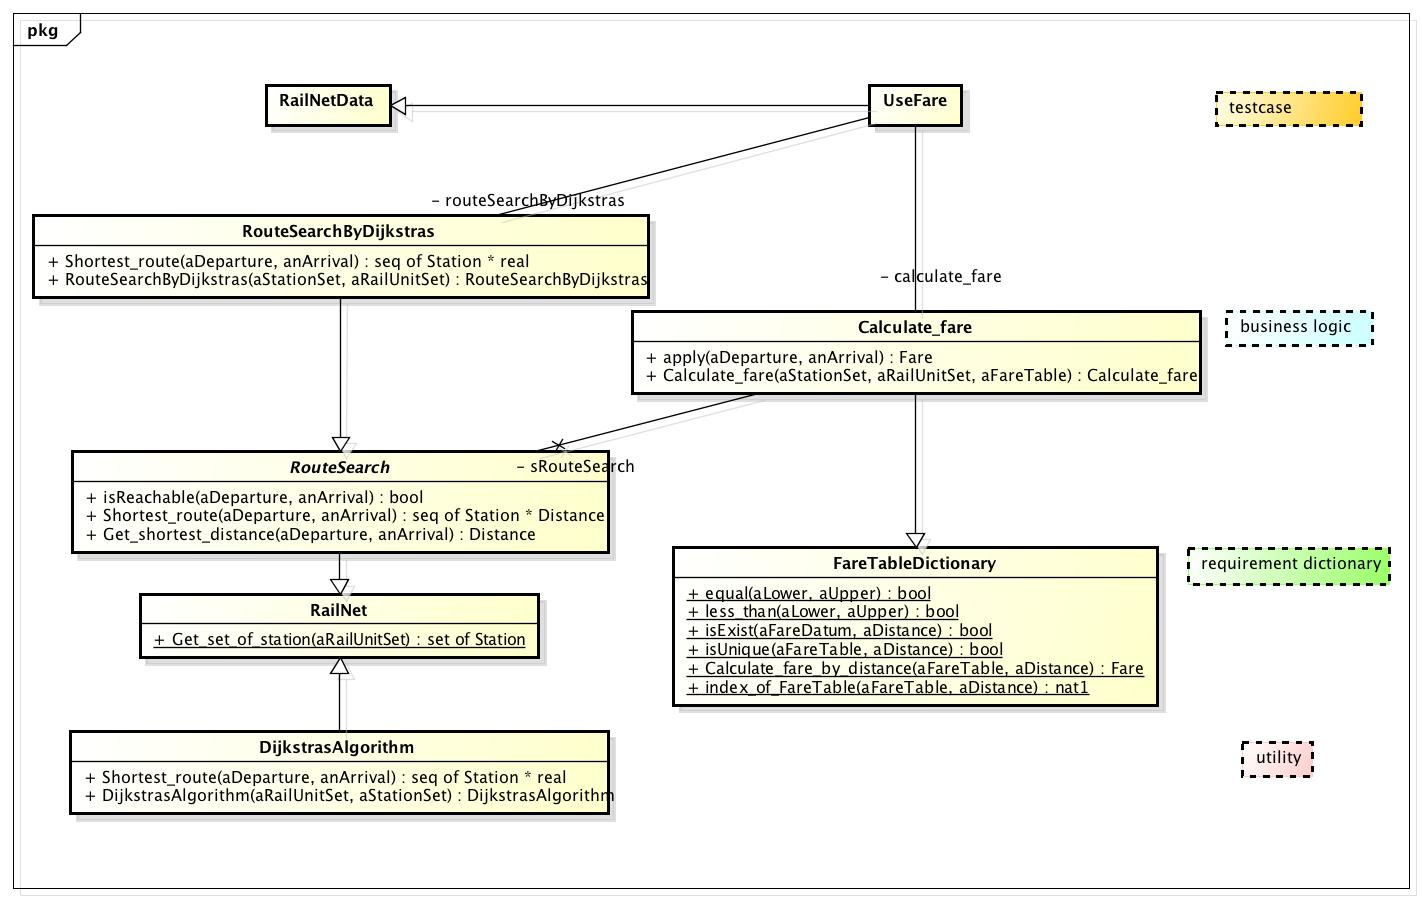
\includegraphics[width=50zw, keepaspectratio]{image/ClassDiagram1.jpg}}
	\caption{ Class Diagram}
	\label{fig:ClassDiagram}
\end{figure}

%\include{Abstract}
\include{CalcFare.vdmpp}
\include{FareTable.vdmpp}
\include{FareTableDic.vdmpp}
\include{railway_network.vdmpp}
\include{route_search.vdmpp}
\include{route_search_by_dijkstra.vdmpp}
\include{dijkstra.vdmpp}
\include{dijkstra4railway.vdmpp}
\include{railway_netwoprk_data.vdmpp}
\include{route_search_testspec.vdmpp}
\include{MyTest.vdmpp}
\include{MyTestCase.vdmpp}
%\include{utilities.vdmpp}
\include{UseFare.vdmpp}

%\begin{thebibliography}{9}
\section{References、Index}
VDM++\cite{Kyushu2016PPE} is a formal specification description language that extended VDM-SL\cite{Kyushu2016SLE} developed by IBM Vienna Research Center in the mid-1970 and further object oriented extension.
\bibliographystyle{jplain}
%\bibliography{/Users/sahara/svnw/sahara}
\bibliography{/Users/sahara/Dropbox/bib/saharaUTF8}
%\bibliography{/Users/ssahara/svnwork/sahara}

%\end{thebibliography}

%\newpage
\addcontentsline{toc}{section}{Index}
\printindex

\end{document}
